% Harrison Zafrin
% DSTII - Final Paper
% ===========================================
% Template for ICMC 2015 (version2)
% adapted from earlier LaTeX paper templates for the ICMC, SMC, etc...
% ===========================================
%----------------------------------------------------------------------------------------
% PACKAGES AND OTHER DOCUMENT CONFIGURATIONS
%----------------------------------------------------------------------------------------

\documentclass{article}
\usepackage{icmc2015template}
\usepackage{times}
\usepackage{ifpdf}
\usepackage{soul}
\usepackage[english]{babel}
%\usepackage{cite}


%%%%%%%%%%%%%%%%%%%%%%%% Some useful packages %%%%%%%%%%%%%%%%%%%%%%%%%%%%%%%
%%%%%%%%%%%%%%%%%%%%%%%% See related documentation %%%%%%%%%%%%%%%%%%%%%%%%%%
%\usepackage{amsmath} % popular packages from Am. Math. Soc. Please use the 
%\usepackage{amssymb} % related math environments (split, subequation, cases,
%\usepackage{amsfonts}% multline, etc.)
%\usepackage{bm}      % Bold Math package, defines the command \bf{}
%\usepackage{paralist}% extended list environments
%%subfig.sty is the modern replacement for subfigure.sty. However, subfig.sty 
%%requires and automatically loads caption.sty which overrides class handling 
%%of captions. To prevent this problem, preload caption.sty with caption=false 
%\usepackage[caption=false]{caption}
%\usepackage[font=footnotesize]{subfig}

% ====================================================
% ================ Define title and author names here ===============
% ====================================================
%user defined variables
\def\papertitle{Intelligent Equalization on Multi-tracks Using Yule-Walker for Spectral Matching}
\def\firstauthor{Harrison Zafrin}
\def\secondauthor{Second Author}
\def\thirdauthor{Third Author}
\def\fourthauthor{Fourth Author}
\def\fifthauthor{Fifth Author}
\def\sixthauthor{Sixth Author}

% adds the automatic
% Saves a lot of ouptut space in PDF... after conversion with the distiller
% Delete if you cannot get PS fonts working on your system.

% pdf-tex settings: detect automatically if run by latex or pdflatex
\newif\ifpdf
\ifx\pdfoutput\relax
\else
   \ifcase\pdfoutput
      \pdffalse
   \else
      \pdftrue
\fi

\ifpdf % compiling with pdflatex
  \usepackage[pdftex,
    pdftitle={\papertitle},
    pdfauthor={\firstauthor, \secondauthor, \thirdauthor},
    bookmarksnumbered, % use section numbers with bookmarks
    pdfstartview=XYZ % start with zoom=100% instead of full screen; 
                     % especially useful if working with a big screen :-)
   ]{hyperref}
  %\pdfcompresslevel=9

  \usepackage[pdftex]{graphicx}
  % declare the path(s) where your graphic files are and their extensions so 
  %you won't have to specify these with every instance of \includegraphics
  \graphicspath{{./figures/}}
  \DeclareGraphicsExtensions{.pdf,.jpeg,.png}

  \usepackage[figure,table]{hypcap}

\else % compiling with latex
  \usepackage[dvips,
    bookmarksnumbered, % use section numbers with bookmarks
    pdfstartview=XYZ % start with zoom=100% instead of full screen
  ]{hyperref}  % hyperrefs are active in the pdf file after conversion

  \usepackage[dvips]{epsfig,graphicx}
  % declare the path(s) where your graphic files are and their extensions so 
  %you won't have to specify these with every instance of \includegraphics
  \graphicspath{{./figures/}}
  \DeclareGraphicsExtensions{.eps}

  \usepackage[figure,table]{hypcap}
\fi

%setup the hyperref package - make the links black without a surrounding frame
\hypersetup{
    colorlinks,%
    citecolor=black,%
    filecolor=black,%
    linkcolor=black,%
    urlcolor=black
}


% ====================================================
% ================ Title and author info starts here ===============
% ====================================================
% Title.
% ------
\title{\papertitle}

% Authors
% Please note that submissions are anonymous, therefore 
% authors' names should not be VISIBLE in your paper submission.
% They should only be included in the camera-ready version of accepted papers.
% uncomment and use the appropriate section (1, 2 or 3 authors)
%
% Single address
% To use with only one author or several with the same address
% ---------------
\oneauthor
{\firstauthor} {NYU \\ %
     {\tt \href{mailto:hzz200@nyu.edu}{hzz200@nyu.edu}}}

%----------------------------------------------------------------------------------------
% BEGIN DOCUMENT
%----------------------------------------------------------------------------------------
\begin{document}

\capstartfalse
\maketitle
\capstarttrue

%----------------------------------------------------------------------------------------
% ABSTRACT AND KEYWORDS
%----------------------------------------------------------------------------------------
\begin{abstract}
In this paper, intelligent equalization is implemented using a dynamic IIR filter where the coefficients are generated via the Yule-Walker method.  While in previous research this technique was shown to be an effective form of intelligent mastering, the goal of this paper is to test these methods in a multi-track setting for future implementation in autonomous mixing systems.  In this off-line MATLAB implementation, audio examples are provided to show the result of filtering, and the spectras are compared to objectivley observe the results.  To look at the code used to run this experiment, visit https://github.com/bombsandbottles/Intelligent-Equalization.
\end{abstract}


%----------------------------------------------------------------------------------------
% INTRODUCTION
%----------------------------------------------------------------------------------------
\section{Introduction}
\label{sec:Introduction}

The spectral response of a sound/recording is highly correlated with genre/instrument type with the data supporting the existence of idealized target frequency responses that professional engineers uniformly conform to \cite{pestana2013spectral}.  With this in mind, it is often the plight of novice audio engineers to achieve these idealized spectral distributions.  This is because mixing as a whole is notoriously difficult, requiring years of experience, expert taste, and fine tuned hearing.  Therefore, the goal of this research is to eliminate this struggle, and shift the focus back to writing phenomenal music by autonomously employing best practices in sound engineering.

Autonomous mastering has already made it to market in the form of Landr (https://www.landr.com/), an on-line tool which uses techniques not foreign to those discussed in this paper and past research \cite{ma2013implementation}.  However while past research was focused on using intelligent equalization as a mastering tool, this paper is focused on testing it on a stem by stem basis.  Consider the following example:  An engineer has a vocal that is ``muddy'' in its spectral character, lacking the polish it needs to stand out as a well engineered stem.  With the technology presented in this paper, the engineer can choose a preset EQ curve of which his unprocessed vocal can morph based on genre/instrument type, instantly giving his vocal ``brilliance'', conforming it to industry standards.

The ideal situation just presented is tested in this paper.  The following vocal stems were analyzed to form an idealized top-40 female pop vocal: [Britney Spears - Break The Ice, Christina Aguilera - Your Body, Katy Perry - Firework, Katy Perry - ET, Kesha - Die Young].  An unprocessed female vocal stem is then run through a time-varying filter to match the target spectra dictated by this genre/instrument type.

%----------------------------------------------------------------------------------------
% ALGORITHM AND IMPLEMENTATION
%----------------------------------------------------------------------------------------
\section{Algorithm and Implementation}\label{sec:Algorithm and Implementation}

In this section, the process on how to perform intelligent equalization using dynamic IIR filtering is detailed.  In summation, the process can be broken down into the following steps: First, a target/idealized frequency response for which our analyzed audio will be morphed to is acquired via the averaging of multiple magnitude spectra.  Once we have our target equalization curve, a transfer function is created on a frame by frame basis through the comparison of our target equalization curve spectra and the incoming audio.  Using the Yule-Walker method, the resulting transfer function from the magnitude spectra comparison is converted into a set of IIR filter coefficients.  The transfer functions across frames are smoothed to provide a sense of cohesion, and the filter is applied via a difference equation.

% CREATING THE TARGET SPECTRA
%----------------------------------------------------------------------------------------
\subsection{Creating the Target Spectra}
\label{subsec:Creating the Target Spectra}

To create the target spectra, the method used in \cite{pestana2013spectral} is implemented.  Using this method, we perform a 4096 point STFT on an audio stem such that it results in a $K \times T$ matrix where $K$ is the frequency bin number and $T$ is the frame number across time.  This matrix known as $X(k,\tau)$ is then averaged across $\tau$ to give the mean frequency response of the individual audio stem.  We opt for a 50\% overlap between frames with a hanning window:

\begin{equation}
\bar{X}(k) = \frac{\sum_{\tau}|X(k,\tau)|}{\left(\frac{x_{len}}{w_{len}}\right)+1}
\label{eq:mean_freq}
\end{equation}

To account for differences in the magnitudes between audio files, normalization is performed on each averaged spectra in the dataset such that the frequency bin sum is 1:

\begin{equation}
\tilde{X}(k) = \frac{\bar{X}(k)}{\sum_{k}\bar{X}}
\label{eq:spectra_normalize}
\end{equation}

And then converted into a cumulative distribution function across the bins:

\begin{equation}
X_c(k) = \sum_{i=0}^{k}\tilde{X}(i)
\label{eq:cumulativesum}
\end{equation}

After concatenating each cumulative distribution $X_c$ into the matrix $X_c(k,n)$ where $N$ is the number of tracks contributing to the target curve, a mean calculation is performed on each cumulative distribution $(\overline{X_c(k)})$.  From here, the overall average spectrum across all tracks can be computed as the difference between adjacent averaged cumulative distributions multiplied by the average magnitude of all tracks in the dataset $S$:

\begin{equation}
\bar{X}_{AV}(k) = \frac{\sum_{k}\bar{X}(k)}{S}\left(\overline{X_c(k)}-\overline{X_c(k-1)})\right)
\label{eq:averagespectrum}
\end{equation}

The resulting target equalization curve can be seen in figure \ref{fig:target}.  As recommended by the literature in \cite{ma2013implementation}, a 17-point moving average filter is applied to the spectrum at only the frequencies above 200hz.  The smoothed version of the spectra is used as the target curve in this experiment. 

\begin{figure}[htbp]
\centering
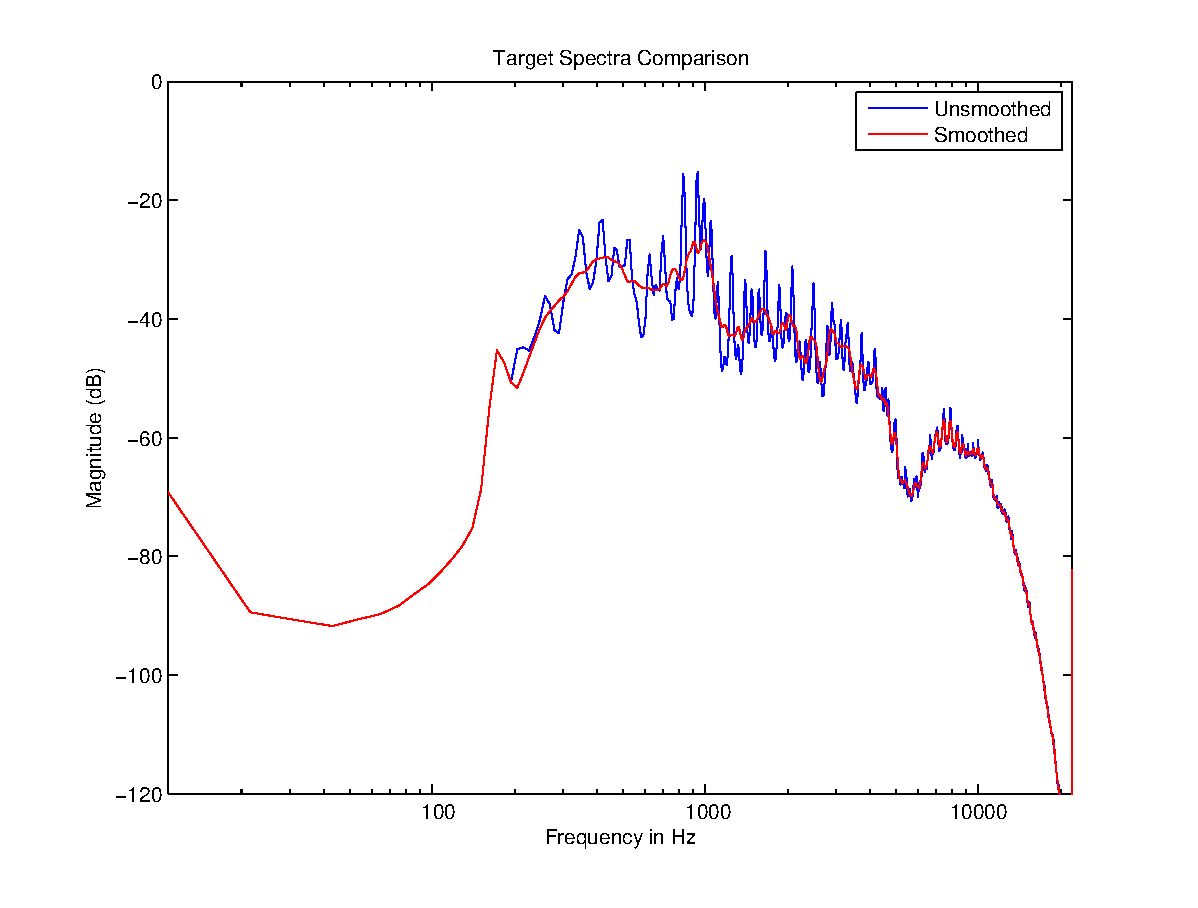
\includegraphics[width=0.9\columnwidth]{targetcurve.eps}
\caption{Target equalization curve for a top-40 female pop vocal.}
\label{fig:target}
\end{figure}

% HYSTERESIS NOISE GATE
%----------------------------------------------------------------------------------------
\subsection{Hysteresis Noise Gate and Loudness Measurement}
\label{subsec:ysteresis Noise Gate and Loudness Measurement}

In an effort to save computational cost and avoid undesirable transfer functions generated from silence, a hysteresis noise gate in conjunction with the ITU-R BS.1770 loudness measurement is implemented to detect active frames.  In this loudness calculation, the signal is preemptively filtered to emulate the frequency response of the human ear before a subsequent modified RMS measurement.  The filter coefficients for a 48khz sampling rate are outlined in the original publication \cite{rec2006bs}, while a formula to calculate the coefficients for different sampling rates is given here \cite{mansbridge2012implementation}.  These filters can be easily implemented in MATLAB by supplying the proper filter coefficients to the \texttt{filt()} function. 

While the ITU-R BS.1770 standard was devised with mastered programmes in mind, autonomous mixing systems have been using it to quantify fader position coefficients.  Therefore, post K-filtering, the loudness for a given track $m$ is calculated by the following equation:

\begin{equation}
\label{eq:ITU-R BS.1770}
L_m[n] = 0.691 \cdot 10log_{10} \cdot \left(\frac{1}{N}\sum_{n=0}^{N-1}xg_m^2[n]\right)
\end{equation}

Here we see a mean-squaring operation is performed across an $N$ long frame of audio where $N$ represents 3 seconds in samples.  The resulting value is converted to dB and the corresponding LU unit is loaded into the loudness vector $L_m$.  In this experiment, the window size of our audio corresponds to the window size of our subsequent spectral analysis (4096 point).  Therefore, in order to simulate the smoothness of a 3 second window, an exponential moving average filter is applied to our resulting $L_m$ vector as in \cite{mansbridge2012implementation}.  The following exponential moving average filter is used in this experiment with an $\alpha$ value of 0.9 based on empirical experimentation:

\begin{equation}
\label{eq:EMAloudness}
y[n] = (\alpha \cdot y(n-1)) + (1-\alpha) \cdot x(n)
\end{equation}

Finally, a hysteresis noise gate is applied with the thresholds of -25 and -30 LUFS to determine whether or not a frame is active.  Active frames will be analyzed to generate a transfer function for filtering, while inactive frames will take on the transfer function of the previous active frame to provide continuity in the changing of filter states.

% SPECTRAL ANALYSIS
%----------------------------------------------------------------------------------------
\subsection{Spectral Analysis}
\label{subsec:Spectral Analysis}

The to-be equalized audio is analyzed in the same fashion as the target EQ curve.  Therefore, a 4096 point FFT is performed with a hanning window and 50\% overlap between frames.  Since the resulting magnitude spectrum will appear in the denominator of the IIR design, problems may arise if values are too small.  Therefore, magnitudes below 0.0001 are either set to 0 or converted to 0.0001 based on empirical experiments.

% OBTAIN DESIRED MAGNITUDE RESPONSE
%----------------------------------------------------------------------------------------
\subsection{Obtain Desired Magnitude Response}
\label{subsec:Obtain Desired Magnitude Response}

To obtain the desired magnitude response per frame, the following calculation is performed:

\begin{equation}
\label{eq:targetmag}
|H_d(\omega)| = \frac{|T(\omega)|}{|X(\omega)|}, \quad \omega \in (0,\pi)
\end{equation}

Here our target magnitude spectrum $|T(\omega)|$ is divided by our active frame $|X(\omega)|$ at the following frequencies: 0, 20, 25, 31.5, 40, 50, 63, 80, 100, 125, 160, 200, 250, 315, 400, 500, 630, 800, 1000, 1250, 1600, 2000, 2500, 3150, 4000, 5000, 6300, 8000, 10000, 12220, 16000, 22050.  The resulting division allows us to compress the amount of information into 33 points yielding us our desired transfer function per frame known as $|H_d(\omega)|$.  $|H_d(\omega)|$ is subsequently normalized for each frame such it lies between 0 and 1 to prevent overshooting.

% FILTER CURVE SMOOTHING
%----------------------------------------------------------------------------------------
\subsection{Filter Curve Smoothing}
\label{subsec:Filter Curve Smoothing}

Since our transfer function $|H_d(\omega)|$ is dependent on the incoming active frame, large changes in the frequency response of adjacent frames can lead to unpleasant sonic results.  Therefore, to provide a sense of cohesion between changing filter states, an exponential moving average filter is applied to $|H_d(\omega)|$ with an $\alpha$ value of 0.9 based on empirical experiments:

\begin{equation}
\label{eq:EMAFILTERCURVE}
H_d'(\omega_{n}) = \alpha \cdot H_d'(\omega_{n-1}) + (1-\alpha) \cdot H_d(\omega_{n})
\end{equation}

% IIR COEFFICIENTS VIA YULE WALKER
%----------------------------------------------------------------------------------------
\subsection{Obtaining IIR Coefficients Using the Yule-Walker Method}
\label{subsec:Obtaining IIR Coefficients Using the Yule-Walker Method}

The Yule-Walker method \cite{friedlander1984modified} is used to perform a least-squares fitting to the desired frequency response $|H_d(\omega)|$ for the active frame.  Due the complexity of the math behind the Yule-Walker method, the MATLAB function \texttt{yulewalk()} was used to generate a 16th order recursive IIR filter with coefficients B and A that best approximate the target frequency response:

\begin{equation}
\label{eq:IIRfilter1}
\frac{B(z)}{A(z)} = \frac{b(0) + b(1) \cdot z^{-1} + \cdots + b(n) \cdot z^{-n}}{1 + a(1) \cdot z^{-1} + \cdots + a(n) \cdot z^{-n}}
\end{equation}

% APPLYING THE FILTER
%----------------------------------------------------------------------------------------
\subsection{Applying The Filter}
\label{subsec:Applying The Filter}

In this MATLAB implementation, the \texttt{filt()} function cannot be used as it does not have a memory of previous $x$ and $y$ values for each frame.  Therefore, a manual filtering is implemented via the following difference equation:\\

% \begin{equation}
\begin{multiline}
% \label{eq:applyfilter}
$y[n] = b(1) \cdot x[n] + b(2) \cdot x[n-1] + \cdots + b(17) \cdot x[n-16] - \\
a(2) \cdot y[n-1] - \cdots - a(17) \cdot y[n-16]$\\
\end{multiline}
% \end{equation}

\\To accomplish this, two buffers are created such that the previous 16 values of $x[n-1]$ to $x[n-16]$ and $y[n-1]$ to $y[n-16]$ can be stored and updated across frames.

%----------------------------------------------------------------------------------------
% RESULTS
%----------------------------------------------------------------------------------------
\section{Results}
\label{sec:Results}

As can be seen in figures \ref{fig:vocal} and \ref{fig:whitenoise}, objective results from the experiment show that the algorithm in its current form is not functioning correctly.  It is possible this can be attributed to the simplified implementation of section \ref{subsec:Obtaining IIR Coefficients Using the Yule-Walker Method}.  In the original implementation of this approach on mixed 2-tracks \cite{ma2013implementation}, the frequencies discussed are centered frequencies, implying a summation of energy across multiple bins to represent perceptual human hearing.  Unfortunately due to the limitations of the \texttt{yulewalk()} function, this was not able to be correctly implemented in time.

Also simplified is the implementation of filter-curve smoothing in section \ref{subsec:Filter Curve Smoothing} of which an empirically attained value of 0.9 was used for $\alpha$ to achieve the most sonically pleasing result.  In this case, vagueness in the literature prevented proper implementation.  For the sake of observing what is possible with a working algorithm, please see \cite{ma2013implementation}.

\begin{figure}[htbp]
\centering
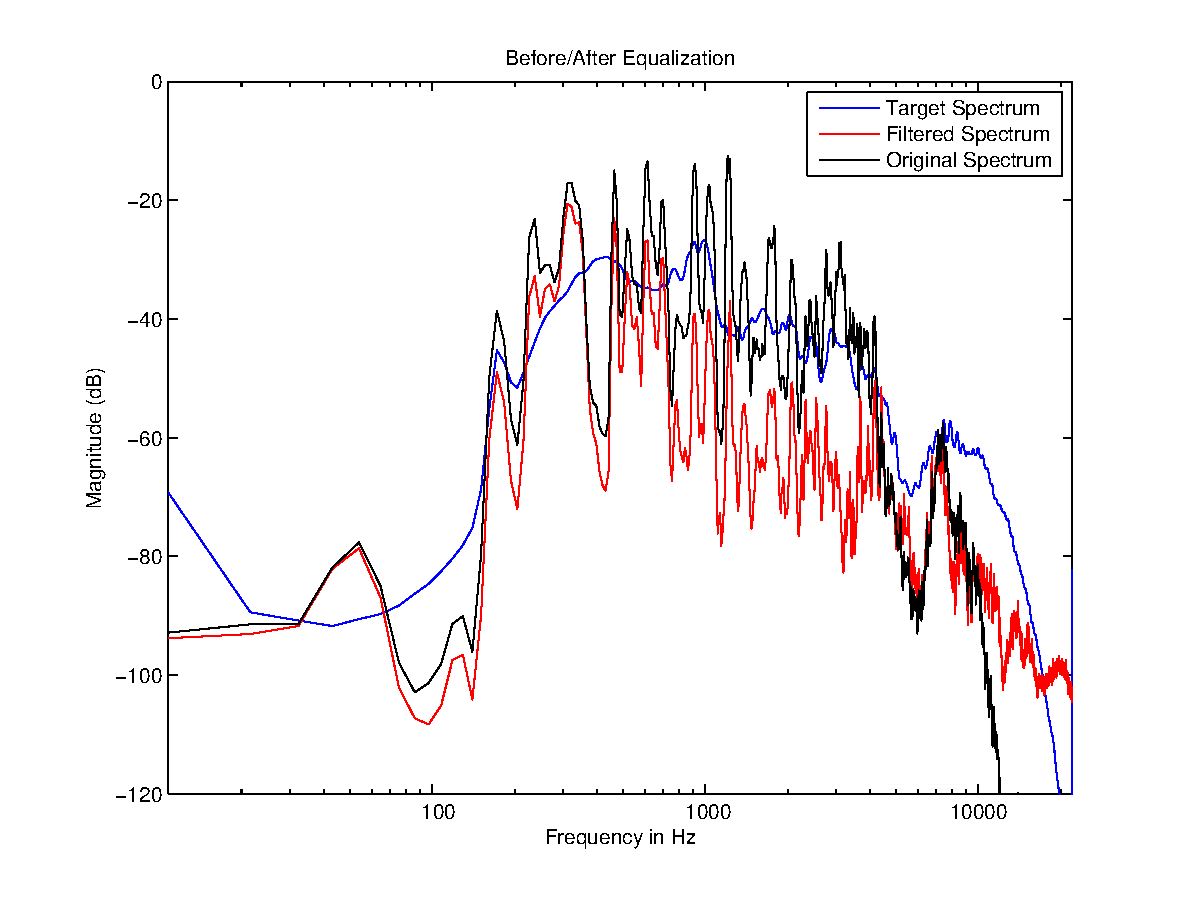
\includegraphics[width=0.9\columnwidth]{vocalresults.eps}
\caption{Equalization results for a female pop vocal.}
\label{fig:vocal}
\end{figure}

% \begin{figure}
% \centering
% 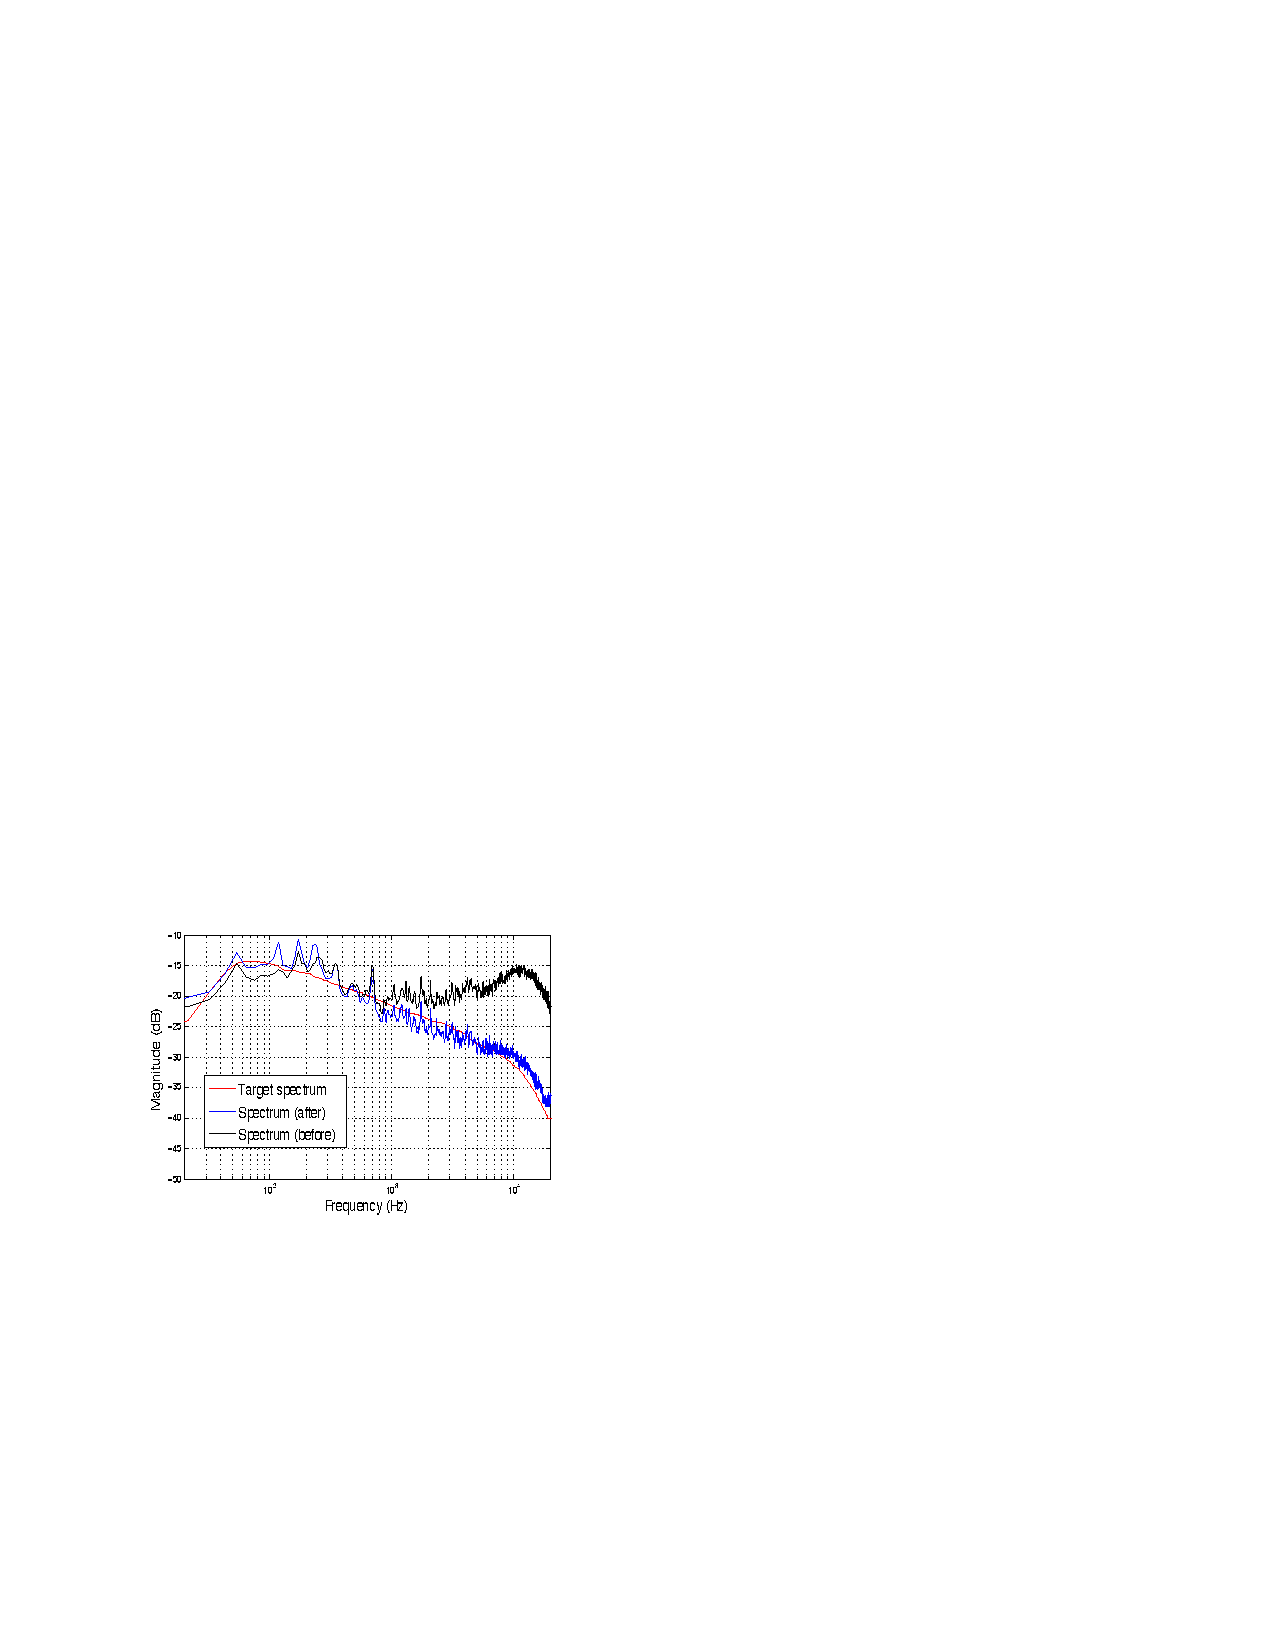
\includegraphics[width=0.9\columnwidth]{Yulewalker.pdf}
% \caption{Prior working implementation on a mixed 2-track.}
% \label{fig:correct}
% \end{figure}

%----------------------------------------------------------------------------------------
% Conclusion
%----------------------------------------------------------------------------------------
\section{Conclusion}
\label{sec:Results}

While a target equalization curve based on genre/instrument type was extracted successfully, its use within a time-varying filter as intelligent equalization was not implemented correctly.  Despite the objective results, subjective listening of the output audio examples warrants future research and further adjustment to the code.  The processed female vocal stem exhibits an enhanced spectral character in the upper frequencies, giving it a bright and shimmery pop vocal sound.  Future research can focus on the idea of time-varying filter states based on amplitude.  For example, quieter played parts exhibit a different spectral envelope than those which are played with intensity.  Measurements in magnitude within the upper frequencies as well as an amplitude gating mechanism can serve to capture different spectral envelopes for different performance intensities.  This would add a sense of dynamics to the time-varying filter instead of keeping its spectral response constant through the duration of a song.  It is also necessary to train the target equalization curve with more data.  In this experiment, only 5 stems were used as reference, where as previous research utilizes a sample size of 600.  Despite these drawbacks, the author believes that the data and methods presented here are convincing enough to pursue further, and looks forward to future developments in the field.

\begin{figure}[htbp]
\centering
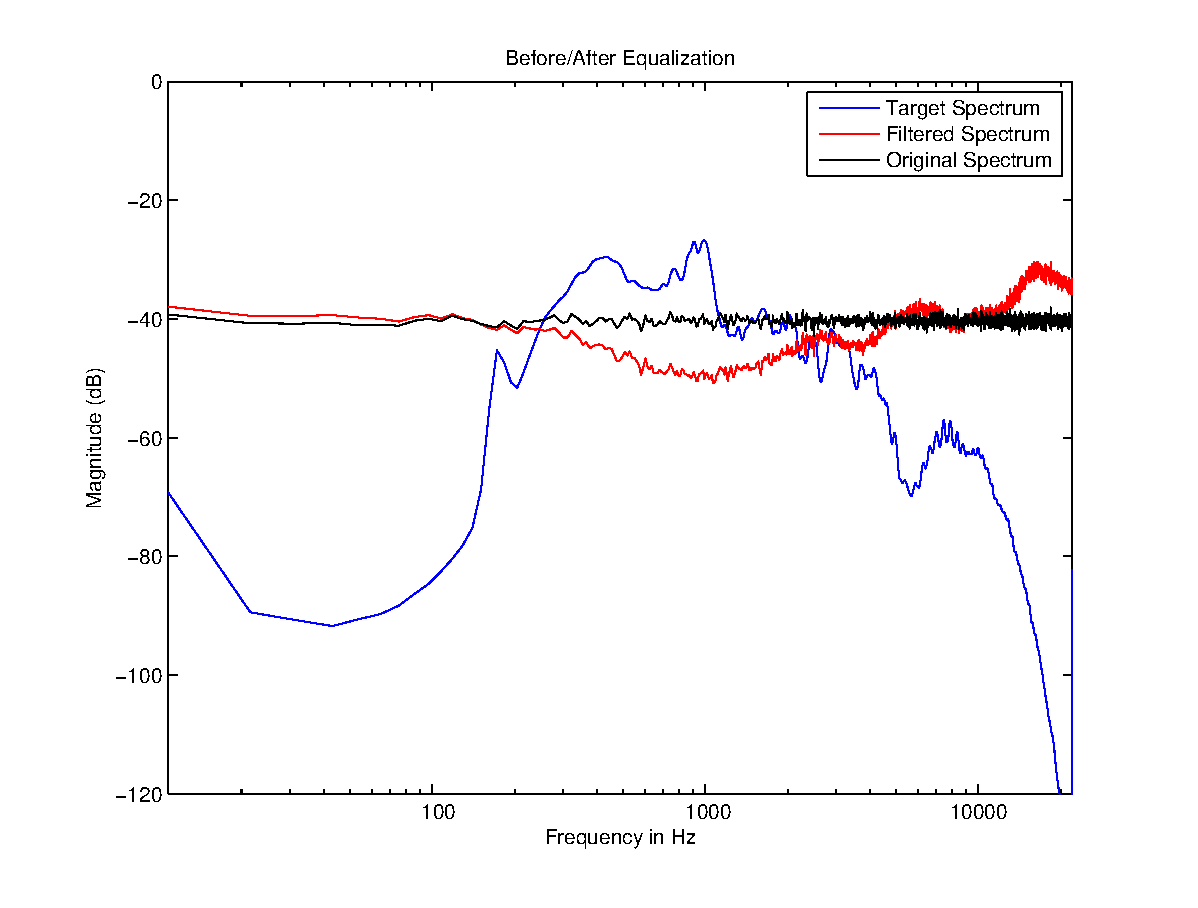
\includegraphics[width=0.9\columnwidth]{whitenoise.eps}
\caption{Equalization results on a white noise test.}
\label{fig:whitenoise}
\end{figure}


%----------------------------------------------------------------------------------------
% Bibliography
%----------------------------------------------------------------------------------------
\bibliography{Zafrin_Harrison_DSTII_FP}

\end{document}
